%	\title[Algebraic Language for the Efficient Representation of Quantum Circuits]{Algebraic Language for the \\ Efficient Representation of Quantum Circuits}



\section{abstract}
    The use of graphical language in quantum computing for the representation of algorithms, although intuitive, is not very useful for different tasks such as the description of quantum circuits in text environments, the calculation of quantum states or the optimization of quantum circuits. While classical circuits can be represented either by circuit graphs or by Boolean expressions, quantum circuits have until now predominantly been illustrated as circuit graphs because no formal language for quantum circuits that allows algebraic manipulations has so far been accepted. This work proposes a means to represent quantum circuits in a convenient and concise manner, similar to the way Boolean expressions are used in classical circuits. The proposed notation allows the consistent and parameterized description of quantum algorithms, as well as the easy handling of the elements that compose it to achieve powerful optimizations in the number of gates of the circuits. To visualize it, a software implementation of an algebraic quantum circuit framework has been made, which allows describing quantum circuits, as well as their respective state vectors, using the proposed algebraic language.

\section{Introduction}

Quantum circuits, pioneered by Deutsch in~\cite{Deutsch1989}, are widely acknowledged as a practical and commonly used approach for illustrating the operations of quantum gates on qubits, ultimately describing the unitary matrix of a quantum computer through graphical representations. Consequently, quantum algorithms and protocols are typically depicted in the format of quantum circuits. This leads to a challenge when dealing with complex quantum algorithms or protocols, as their circuit graphs can quickly surpass manageable sizes, making drawing and manipulation impractical.

In classical computing, circuits can be not only graphically represented but also expressed as Boolean expressions using Boolean gates that implement logic based on truth tables. These Boolean expressions are well-suited for algebraic manipulations. Conversely, the derivation of an algebraic expression for a quantum circuit has been challenging because quantum computing lacks a language analogous to Boolean expressions in classical computing. The present paper aims to introduce a formal semantics for a novel algebraic language designed to streamline the expression of quantum circuits in a concise manner so that fundamental algebraic laws for quantum circuits can be easily proven, and complex quantum algorithms can be simplified when expressed in this language.

A bibliographic review shows the great interest that the problem arouses, although no solution has been fully accepted to date.

In the work~\cite{gerdt}, a Mathematica package is presented for the simulation of quantum computing based on the circuit model, providing an interface to specify and draw a quantum circuit and to build the corresponding unitary matrix for quantum computing defined by the circuit.
Another method for representing the unitary matrix of a quantum circuit as an algebraic equation is presented in the paper~\cite{Hutsell}.
Note that the present work does not require the use of Mathematica or matrices.

Another close paper is~\cite{Ying}, which presents the design of an algebraic language for formally specifying quantum circuits in distributed quantum computing so that using that language, quantum circuits can be represented in a compact way. However, the language proposed in the present work is simpler and closer to simulation programming, which facilitates its implementation. Indeed, this issue is demonstrated through the presentation of a first version of a software implementation of the proposal. In particular, the present notation proposal is more intuitive as it sets the quantum gates in order of execution (from left to right).

The equational theory of quantum circuits is discussed in the paper~\cite{Staton}, which presents an axiomatization of the relationship between measurement, qubit initialization and a set of unitary gates. Another recent work~\cite{Wang19} proposes the unification of quantum and classical computing in open quantum systems.
Also recently, the paper~\cite{doi:10.1098/rsta.2019.0161} describes the flow of quantum compilation with several NP-hard tasks and proposes algorithms based on Boolean satisfiability to address those computationally complex problems. Note that the three  aforementioned recent papers address related but different topics than the one addressed in the present paper.

Finally, one of the latest related  works is~\cite{Wang21} on the equivalence of dynamic quantum circuits. That proposal looks promising, but has only been evaluated on toy examples, with no available software packages for  checking yet.

This paper is structured as follows. Section 1 provides a brief introduction to the topic. Section 2 describes the first basic notations for states and gates.  Section 3 includes several  general basic properties  while Section 4 focuses on specific properties of the controlled Pauli-\gate{X} gate. Section 5 introduces a first software implementation that makes use of the proposed language.
Section 6 shows the usefulness of the proposed language by demonstrating a use case that   illustrates an effective circuit simplification based on the introduced notation.
Finally, Section 7 closes this paper with some conclusions and future work.

\section{Preliminaries}
The fundamental information unit within a quantum computing system is the qubit, which is denoted by a unitary vector within a Hilbert space of dimension 2.
Multiple qubits can be taken together so that an element of the Hilbert space of $n$ qubits is considered. This case can be seen as the tensor product of the $n$ Hilbert spaces corresponding to each qubit in the system, so that the resulting space dimension is $2^n$.

Let $\mathbb{N}$ and $\mathbb{C}$ denote the sets of natural and complex numbers, respectively. The notation $\mathbb{N}_n$ is used to denote the subset of $\mathbb{N}$ that contains the natural numbers smaller or equal than $n$.
In set theory, for any finite set $S$, its number of elements  $|S|$ is called the cardinality of $S$.

\subsection{Kets}

As introduced in~\cite{diracBraket},  qubits are normally written in the so-called bra–ket notation.

On the one hand, each qubit is represented as a ket, of the form $\ket{a}$,  which denotes a vector $a$ in a vector space $V$.
For instance, the computational basis states are written  as $\ket{0}$ and $\ket{1}$, and called ket 0 and ket 1, respectively (see~\cite{Nielsen_Chuang_2010}).
Thus, any qubit can be described by a linear combination of these two basis states as $\ket{a} =\alpha_0\ket{0} +\alpha_1 \ket{1}$, where $\alpha_0,  \alpha_1 \in \mathbb{C}$ such that $ |\alpha_0|^{2}+|\alpha_1|^{2}=1$.

On the other hand, a bra is of the form $\bra{f}$ and denotes a linear form $f$ that represents a linear map that maps each vector in $V$
to a number in $\C$.

In this way,  when the function $\bra{f}$ acts on a vector $\ket{a}$, the result  is written as $\braket{f}{a}$.

\begin{notation}
    For any qubit $\ket{a_k}=\alpha_{k0}\ket{0} +\alpha_{k1} \ket{1}$, the following notation is used:
    $\alpha_{k0}=\braket{a_k}{0}$ and $\alpha_{k1}=\braket{a_k}{1}$.
\end{notation}

For example, for two qubits $\ket{a_1}$ and $\ket{a_2}$, the following can be written:
\begin{align}
    \label{eq:2qubit-coordenadas}
    \ket{a_1a_2}&=\alpha_{10}\ket{0a_2}+\alpha_{11}\ket{1a_2}=\\
    &=\alpha_{20}\ket{a_10}+\alpha_{21}\ket{a_11}=\\
    &=\alpha_{10} \alpha_{20}\ket{00}+\alpha_{10} \alpha_{21}\ket{01}+\alpha_{11} \alpha_{20}\ket{10}+\alpha_{11} \alpha_{21}\ket{11}.
\end{align}

In general, for $n$ qubits $\ket{a_1}\dots\ket{a_n}$, the composite ket  $\ket{a}=\ket{a_1\cdots a_n}$  can be written as shown below:
\begin{equation}
    \label{eq:nqubit-coordenadas}
    \ket{a}=\alpha_{k0}\ket{a_1\cdots a_{k-1}0a_{k+1}\cdots a_n}+\alpha_{k1}\ket{a_1\cdots a_{k-1}1a_{k+1}\cdots a_n}.
\end{equation}

\begin{notation}
    For any ket $\ket{a}=\ket{a_1\dots a_n}$ of $n$ qubits, the following notation is used:
    $\stateket{a}{k}{u} = \ket{a_1\cdots a_{k-1}u a_{k+1}\cdots a_n}$, where $k \in \mathbb{N}_n$ and $u\in\set{0,1}$.
\end{notation}

Consequently, the expression~(\ref{eq:nqubit-coordenadas}) can be written as follows:
\begin{equation}
    \label{eq:canonical-state}
    \ket{a}= \alpha_{k0}\stateket{a}{k}{0}+\alpha_{k1}\stateket{a}{k}{1}.
\end{equation}

For instance, if $\ket{a_1},\ket{a_2}$ and $\ket{a_3}$ are three qubits, then:
\begin{itemize}
    \item $\stateket{a_1}{1}{0}=\ket{0}$ and $\stateket{a_1}{1}{1}=\ket{1}$.
    \item $\stateket{a_1 a_2}{2}{0}=\ket{a_1 0}$.
    \item $\ket{a_1 a_2 a_3}=\alpha_{20}\ket{a_1 0 a_3}+\alpha_{21}\ket{a_1 1 a_3}=\alpha_{20}\stateket{a}{2}{0}+\alpha_{21}\stateket{a}{2}{1}$.
    \item $\stateket{00a_3}{3}{1}=\ket{001}$.
\end{itemize}

\subsection{Quantum Gates}
A quantum gate is a basic quantum circuit operating on a small number of qubits.

For example, a single-qubit gate $\gate{A}$   can be applied over the first qubit of a ket $\ket{a_1a_2} $ and the result is $\gate{A}\ket{a_1}\otimes \ket{a_2}$. It can also be applied over the last of both qubits and then the result is $\ket{a_1}\otimes \gate{A}\ket{a_2}$.

\begin{notation}
    If $\gate{A}$ is a single-qubit  gate and $\ket{a}=\ket{a_1\cdots a_n}$ is a ket with $n$ qubits, the following notation is used:
    \[\ket{a_1\cdots a_h\gate{A}a_{h+1}\cdots a_n}=\ket{a_1\cdots a_{h-1}}\otimes\gate{A}\ket{a_h}\otimes \ket{a_{h+1}\cdots a_n},\] where $1<h<n$.
\end{notation}
For example, if $\ket{a}=\ket{a_1a_2}$ then
$\ket{a_1\gate{A}a_2} = \gate{A}\ket{a_1}\otimes \ket{a_2}$ and $\ket{a_1a_2\gate{A}} =\ket{a_1}\otimes \gate{A}\ket{a_2}$.

\begin{notation}
    The effect over the $k$-th qubit of the  ket $\ket{a}=\ket{a_1\cdots a_n}$ of the quantum gate $\gate{A}$ can be denoted by:  $\ket{a}\gate{A}_k=\stateket{a}{k}{\gate{A}}$.
\end{notation}

\begin{notation}
    For any set $\Gamma=\set{l_1,\dots,l_h}\subseteq\mathbb{N}_n$ and any single-qubit gate $\gate{A}$, the following notation is used:
    \begin{align}
        \gate{A}_{\Gamma} &= \gate{A}_{l_1,\dots,l_h}=\\
        &=\prod_{k\in\Gamma}\gate{A}_k
    \end{align}
\end{notation}

Note that, according to the previous notation, for the specific case of the empty set $\Gamma=\emptyset$, the resulting quantum gate is the identity gate $\gate{A}_\Gamma=\gate{I}$.

In conclusion, for example,  the action of a single-qubit gate $\gate{A}$ over the ket $\ket{a}=\ket{a_1a_2}$ can be expressed using four distinct forms:
\begin{equation*}
    \gate{A}\ket{a_1}\otimes \ket{a_2} = \ket{a_1\gate{A}a_2}= \ket{a_1a_2}\gate{A}_1= \stateket{a_1a_2}{1}{\gate{A}}
\end{equation*}

\subsection{Pauli Gates}
The well-known Pauli gates $\gate{I}, \gate{X}, \gate{Y}, \gate{Z}$ can be expressed according to the  notation  introduced above as follows:
\begin{align}
    \ket{a}\gate{I}_k &= \alpha_{k0}\stateket{a}{k}{0}+\alpha_{k1}\stateket{a}{k}{1} \\
    \ket{a}\gate{X}_k &= \alpha_{k0}\stateket{a}{k}{1}+\alpha_{k1}\stateket{a}{k}{0}\\
    \ket{a}\gate{Y}_k &= i \alpha_{k0}\stateket{a}{k}{1}-i \alpha_{k1}\stateket{a}{k}{0}\\
    \ket{a}\gate{Z}_k &= \alpha_{k0}\stateket{a}{k}{0}-\alpha_{k1}\stateket{a}{k}{1}
\end{align}

\subsection{Hadamard Gate}
The Hadamard gate is a well-known single-qubit gate that maps the basis states $\ket{0}$ and $\ket{1}$  to $\ket{+}=\frac{\ket{0}+\ket{1}}{\sqrt{2}}$ and $\ket{-}=\frac{\ket{0}-\ket{1}}{\sqrt{2}}$, respectively.

Thus, the Hadamard gate can be expressed using the introduced notation as follows:
\begin{align}
    \label{eq:hadamard}
    \ket{a}\gate{H}_k&=\alpha_{k0}\ket{a}^{k}_{+}+\alpha_{k1}\ket{a}^{k}_{-}=\\
    &=
    \frac{\alpha_{k0}+\alpha_{k1}}{\sqrt{2}}\ket{a}^{k}_{0}+\frac{\alpha_{k0}-\alpha_{k1}}{\sqrt{2}}\ket{a}^{k}_{1}
\end{align}

\subsection{Controlled Gates}
Controlled gates are applied to kets formed by multiple qubits so that one or more qubits serve as controllers for a specific operation on one or more qubits of the ket.

The simplest controlled gate $\gate{A}$ over a ket $\ket{a}=\ket{a_1\dots a_n}$ has only one control qubit $\ket{a_h}$ and only one target qubit $\ket{a_k}$.

\begin{notation}
    The effect over the  ket $\ket{a}=\ket{a_1\cdots a_n}$ of the controlled gate $\gate{A}$ with control qubit $\ket{a_h}$ and  target qubit $\ket{a_k}$ can be denoted by:
    \begin{align}
        \label{eq:generic-controlled-gate}
        \ket{a}\stategate{A}{h}{k}&=\alpha_{h0}\stateket{a}{h}{0}+\alpha_{h1} \stateket{a}{h}{1}\stategate{A}{}{k}= \\
        &=\alpha_{h0}\stateket{a}{h}{0}+\alpha_{h1} \stateket{a}{hk}{1\gate{A}}
    \end{align}
\end{notation}

\begin{notation}
    The effect over the  ket $\ket{a}=\ket{a_1\cdots a_n}$ of a controlled gate $\gate{A}$ with various control qubits $\Gamma=\set{h_1,\dots,h_l}\subseteq\mathbb{N}_n$  and various target qubits $\Lambda=$ $\text{ }$ $\set{k_1,\dots,k_m}\subseteq\mathbb{N}_n$ can be denoted by:
    $\gate{A}^{\Gamma}_{\Lambda}=\stategate{A}{h_1,\dots,h_l}{k_1,\dots, k_m}$.
\end{notation}
Note that, according to the previous notation, for the specific case of the empty set $\Gamma=\emptyset$, the resulting quantum gate is $\stategate{A}{\Gamma}{\Lambda}=\gate{A}_{\Lambda}$.

\section{General Basic Properties}
Some generic properties of  gates in a quantum circuit are proven below.
\begin{proposition}
    Let $\gate{A}$ be a single-qubit gate such that $\gate{A}\gate{A}=\gate{I}$. Then $\forall h,k \in \mathbb{N}_n$
    \begin{align}
        \label{eq:puerta-involutiva}
        \gate{A}_k\gate{A}_k &= \gate{I}\\
        \stategate{A}{h}{k}\stategate{A}{h}{k} &= \gate{I}
    \end{align}
    .
\end{proposition}
\begin{proof}
    Let $\ket{a}$ be a ket and two indexes $h,k \in \mathbb{N}_n$.
    To prove expression (16):
    \begin{align*}
        \ket{a}\gate{A}_k\gate{A}_k
        &=\stateket{a}{k}{\gate{A}}\gate{A}_k=\ket{a}^k_{\gate{AA}}=\stateket{a}{k}{\gate{I}}=\ket{a}.
    \end{align*}
    Analogously, to prove expression (17), according to~(\ref{eq:generic-controlled-gate}):
    \begin{align*}
        \ket{a}\stategate{A}{h}{k}\stategate{A}{h}{k}
        &=\alpha_{h0}\stateket{a}{h}{0}\stategate{A}{h}{k}+\alpha_{h1}\stateket{a}{hk}{1A}\stategate{A}{h}{k}=\\
        &=\alpha_{h0}\stateket{a}{h}{0}+\alpha_{h1}\stateket{a}{hk}{1AA}=\\
        &=\alpha_{h0}\stateket{a}{h}{0}+\alpha_{h1}\stateket{a}{h}{1}=\ket{a}.
    \end{align*}
\end{proof}

\begin{proposition}
    Let $\gate{A}$ and $\gate{B}$ be two single-qubit gates.
    Then, for any  two  distinct indexes $h,k \in \mathbb{N}_n$
    \begin{equation}
        \label{eq:conmutacion-qubits}
        \gate{A}_k\gate{B}_{h} = \gate{B}_{h}\gate{A}_k
    \end{equation}

\end{proposition}
\begin{proof}
    Let $\ket{a}$ be a ket.
    For any   two distinct indexes $h,k \in \mathbb{N}_n$
    \begin{align*}
        \ket{a}\gate{A}_k\gate{B}_{h}
        &=\stateket{a}{k}{\gate{A}}\gate{B}_{h}=\stateket{a}{kh}{\gate{AB}}=\stateket{a}{h}{\gate{B}}\gate{A}_{k}=\ket{a}\gate{B}_{h}\gate{A}_k.
    \end{align*}
\end{proof}

\begin{proposition}
    Let $\gate{A}$ be a single-qubit gate.
    Then, for any  three distinct indexes $h,k,k^\prime \in \mathbb{N}_n$
    \begin{align}
        \stategate{A}{h}{k}\stategate{A}{h}{k^\prime} &= \stategate{A}{h}{k^\prime}\stategate{A}{h}{k}
    \end{align}
\end{proposition}

\begin{proof}
    Let $\ket{a}$ be a ket.\ For any three distinct  indexes $h,k,k^\prime \in \mathbb{N}_n$:
    \begin{align*}
        \ket{a}\stategate{A}{h}{k}\stategate{A}{h}{k^\prime}
        &=\alpha_{h0}\stateket{a}{h}{0}\stategate{A}{h}{k^\prime}+\alpha_{h1}\stateket{a}{hk}{1\gate{A}}\stategate{A}{h}{k^\prime}=\\
        &=\alpha_{h0}\stateket{a}{h}{0}+\alpha_{h1}\stateket{a}{hkk^\prime}{1\gate{AA}}=\\
        &=\alpha_{h0}\stateket{a}{h}{0}\stategate{A}{h}{k}+\alpha_{h1}\stateket{a}{hk^\prime}{1\gate{A}}\stategate{A}{h}{k}=\\
        &=\ket{a}\stategate{A}{h}{k^\prime}\stategate{A}{h}{k}
    \end{align*}
\end{proof}

\begin{proposition}
    Let $\gate{A}$ and $\gate{B}$ be two single-qubit gates, and $\Gamma, \Lambda \subset \mathbb{N}_n$ be two sets such that $\Gamma\cap\Lambda=\emptyset$.
    Then
    \begin{equation}
        \label{eq:conmutacion-sets}
        \gate{A}_\Gamma\gate{B}_{\Lambda} = \gate{B}_{\Lambda}\gate{A}_{\Gamma}
    \end{equation}
\end{proposition}
\begin{proof}
    Let $\Gamma=\set{h_1,\dots,h_l}$ and $\Lambda=\set{k_1,\dots,k_m}$ be two subsets of $\mathbb{N}_n$. Then
    \begin{align*}
        \gate{A}_{\Gamma}\gate{B}_{\Lambda}=\gate{A}_{\Gamma}\gate{B}_{k_1}\cdots\gate{B}_{k_m}=\gate{A}_{h_1}\cdots\gate{A}_{h_l}\gate{B}_{k_1}\cdots\gate{B}_{k_m}.
    \end{align*}
    Since $\Gamma\cap\Lambda=\emptyset$, then $h_l\neq k_1$. Thus, according to expression (\ref{eq:conmutacion-qubits}), the following is true $\gate{A}_{h_l}\gate{B}_{k_1}=\gate{B}_{k_1}\gate{A}_{h_l}$.
    The same reasoning is valid for all elements of $\Gamma$, so $\gate{A}_{\Gamma}\gate{B}_{k_1}=\gate{B}_{k_1}\gate{A}_{\Gamma}$. Consequently,
    \begin{align*}
        \gate{A}_{\Gamma}\gate{B}_{\Lambda}&=\gate{A}_{\Gamma}\gate{B}_{k_1}\cdots\gate{B}_{k_m}=\gate{B}_{k_1}\gate{A}_{\Gamma}\gate{B}_{k_2}\cdots\gate{B}_{k_m}=\\
        &=\dots = \gate{B}_{k_1}\cdots\gate{B}_{k_m}\gate{A}_{\Gamma}=\gate{B}_{\Lambda}\gate{A}_{\Gamma}
    \end{align*}
\end{proof}

\begin{proposition}
    Let $\gate{A}$ be a single-qubit gate.
    Then, for any two sets $\Gamma, \Lambda \subset \mathbb{N}_n$
    \begin{equation}
        \label{eq:junta-puertas}
        \gate{A}_\Gamma\gate{A}_{\Lambda} = \gate{A}_{\Gamma\cup\Lambda}\gate{A}_{\Gamma\cap\Lambda}
    \end{equation}
    
\end{proposition}
\begin{proof}
    From basic set theory, $\Gamma\cup\Lambda$ can be expressed as $(\Gamma-(\Gamma\cap\Lambda))\cup(\Lambda-(\Gamma\cap\Lambda))\cup(\Gamma\cap\Lambda)$. Then, the following is true
    \begin{align*}
        \gate{A}_{\Gamma}\gate{B}_{\Lambda}&=\prod_{h\in\Gamma}\gate{A}_{h}\prod_{k\in\Lambda}\gate{A}_{k}=\\
        &=\prod_{h\in\Gamma-(\Gamma\cap\Lambda)}\gate{A}_{h}\prod_{h^\prime\in\Gamma\cap\Lambda}\gate{A}_{h^\prime}\prod_{k\in\Lambda-(\Gamma\cap\Lambda)}\gate{A}_{k}\prod_{k^\prime\in\Gamma\cap\Lambda}\gate{A}_{k^\prime}=\\
        &=\prod_{h\in(\Gamma-(\Gamma\cap\Lambda))\cup(\Lambda-(\Gamma\cap\Lambda))\cup(\Gamma\cap\Lambda)}\gate{A}_{h}\prod_{k^\prime\in\Gamma\cap\Lambda}\gate{A}_{k^\prime}=\\
        &=\prod_{h\in\Gamma\cup\Lambda}\gate{A}_{h}\prod_{k^\prime\in\Gamma\cap\Lambda}\gate{A}_{k^\prime}=\gate{A}_{\Gamma\cup\Lambda}\gate{A}_{\Gamma\cap\Lambda}
    \end{align*}
\end{proof}

Below a theoretical result shows that  if a single-qubit gate is applied over a subset of qubits that are eigenstates of the gate  with eigenvalue -1, then the result coincides with that of the result with another subset with the same cardinality parity (see~\cite{Nielsen_Chuang_2010}). On the other hand, if this latter subset has a different cardinality parity, then the result coincides with the product of the first result with the eigenvalue.
\begin{proposition}
    Let $\gate{A}$ be a single-qubit gate. Let $\ket{a}$ be a ket and $\Gamma, \Lambda \subseteq \mathbb{N}_n$ such that $\forall k \in \Gamma \cup \Lambda, \ket{a} \gate{A}_{k} = -\ket{a}$. Then
    \begin{equation}
        \ket{a} \stategate{A}{}{\Gamma} = (-1)^{|\Lambda|-|\Gamma|}\ket{a} \stategate{A}{}{\Lambda}.
    \end{equation}
\end{proposition}
\begin{proof}
    If $\Gamma=\set{k_1,\dots,k_l}$ where $l=|\Gamma|$, then
    \begin{align*}
        \ket{a} \stategate{A}{}{\Gamma} &= \ket{a} \prod_{k \in \Gamma} \gate{A}_k = \ket{a}\gate{A}_{k_1} \stategate{A}{}{k_2}\dots\stategate{A}{}{k_l} =\\
        &= (-1)\ket{a}\gate{A}_{k_2}\dots\stategate{A}{}{k_l} =\dots = (-1)^{|\Gamma|} \ket{a}.
    \end{align*}
    Analogously, $\ket{a} \stategate{A}{}{\Lambda} = (-1)^{|\Lambda|} \ket{a}$.
    Then
    \begin{align*}
        \ket{a} \stategate{A}{}{\Gamma} &= (-1)^{|\Gamma|} \ket{a} = (-1)^{|\Gamma|-|\Lambda|}(-1)^{|\Lambda|} \ket{a}=\\
        &=(-1)^{|\Gamma|-|\Lambda|}\ket{a} \stategate{A}{}{\Lambda}.
    \end{align*}
\end{proof}

\section{Specific Properties of the Controlled Pauli-X Gate}
In this section, some specific properties involving  the controlled Pauli-\gate{X} gate are demonstrated.

\begin{proposition}
    Let $h,k \in \mathbb{N}_n$ be two indexes.
    Then
    \begin{equation}
        \stategate{X}{h}{k}\stategate{Z}{}{k}\stategate{X}{h}{k} = \stategate{Z}{}{h,k}
    \end{equation}
\end{proposition}
\begin{proof}
    If $\ket{a}$ is a ket and $h\neq k\in \mathbb{N}_n$ are two indexes, then
    \begin{align*}
        \ket{a}\stategate{X}{h}{k}\stategate{Z}{}{k}\stategate{X}{h}{k}
        &=\alpha_{h0}\stateket{a}{h}{0}\stategate{Z}{}{k}\stategate{X}{h}{k}+
        \alpha_{h1}\stateket{a}{hk}{1X}\stategate{Z}{}{k}\stategate{X}{h}{k}=\\
        &=\alpha_{h0}\stateket{a}{hk}{0Z}\stategate{X}{h}{k}+
        \alpha_{h1}\stateket{a}{hk}{1ZX}\stategate{X}{h}{k}=\\
        &=\alpha_{h0}\stateket{a}{hk}{0Z}+\alpha_{h1}\stateket{a}{hk}{1XZX}=\\
        &=\alpha_{h0}\stateket{a}{hk}{0Z}-\alpha_{h1}\stateket{a}{hk}{1Z}=\\
        &=\alpha_{h0}\stateket{a}{h}{0}\gate{Z}_k-\alpha_{h1}\stateket{a}{h}{1}\gate{Z}_k=\\
        &=\ket{a}\stategate{Z}{}{h,k}
    \end{align*}
\end{proof}

For the following result it is necessary to introduce the SWAP gate, which acts over two qubits, exchanging the state of both positions:
\begin{align}
    \label{eq:swap}
    \begin{split}
        \ket{a}(SWAP)_{h,k}&=\alpha_{h0}\alpha_{k0}\stateket{a}{hk}{00}+\alpha_{h0}\alpha_{k1}\stateket{a}{hk}{10}+\\
        &+\alpha_{h1}\alpha_{k0}\stateket{a}{hk}{01}+\alpha_{h1}\alpha_{k1}\stateket{a}{hk}{11}
    \end{split}
\end{align}
\begin{proposition}
    Let $h,k \in \mathbb{N}_n$ be two indexes.
    Then
    \begin{equation}
        \stategate{X}{h}{k}\stategate{X}{k}{h}\stategate{X}{h}{k} = \stategate{(SWAP)}{}{h,k}
    \end{equation}
\end{proposition}
\begin{proof}
    If $\ket{a}$ is a ket and $h\neq k \in \mathbb{N}_n$ are two indexes, then 
    \begin{align*}
        \ket{a}\stategate{X}{h}{k}\stategate{X}{k}{h}\stategate{X}{h}{k}
        &=\alpha_{h0}\stateket{a}{h}{0}\stategate{X}{h}{k}\stategate{X}{k}{h}+
        \alpha_{h1}\stateket{a}{hk}{1X}\stategate{X}{h}{k}\stategate{X}{k}{h}=\\
        &=\alpha_{h0}\stateket{a}{h}{0}\stategate{X}{k}{h}\stategate{X}{h}{k}+
        \alpha_{h1}\alpha_{k0}\stateket{a}{hk}{11}\stategate{X}{k}{h}\stategate{X}{h}{k}+\\
        &+\alpha_{h1}\alpha_{k1}\stateket{a}{hk}{10}\stategate{X}{k}{h}\stategate{X}{h}{k}
        =\alpha_{h0}\alpha_{k0}\stateket{a}{hk}{00}\stategate{X}{h}{k}+\\
        &+\alpha_{h0}\alpha_{k1}\stateket{a}{hk}{11}\stategate{X}{h}{k}
        +\alpha_{h1}\alpha_{k0}\stateket{a}{hk}{01}\stategate{X}{h}{k}+\\
        &+\alpha_{h1}\alpha_{k1}\stateket{a}{hk}{10}\stategate{X}{h}{k}
        =\alpha_{h0}\alpha_{k0}\stateket{a}{hk}{00}+\\
        &+\alpha_{h0}\alpha_{k1}\stateket{a}{hk}{10}
        +\alpha_{h1}\alpha_{k0}\stateket{a}{hk}{01}+ \alpha_{h1}\alpha_{k1}\stateket{a}{hk}{11}=\\
        &=\stategate{(SWAP)}{}{h,k}
    \end{align*}
\end{proof}

\begin{proposition}
    Let $h,k \in \mathbb{N}_n$ be two indexes.
    Then
    \begin{equation}
        \gate{H}_{hk}\stategate{X}{k}{h}\gate{H}_{hk} = \stategate{X}{h}{k}
    \end{equation}
\end{proposition}
\begin{proof}
    If $\ket{a}$ is a ket and $h\neq k \in \mathbb{N}_n$ are two indexes, then
    \begin{align*}
        \ket{a}\gate{H}_{kh}\stategate{X}{k}{h}\gate{H}_{kh}
        &=\alpha_{h0}\stateket{a}{h}{+}\gate{H}_k\stategate{X}{k}{h}\gate{H}_{kh} + \alpha_{h1}\stateket{a}{h}{-}\gate{H}_k\stategate{X}{k}{h}\gate{H}_{kh}=\\
        &=\alpha_{h0}\alpha_{k0}\stateket{a}{hk}{++}\stategate{X}{k}{h}\gate{H}_{kh} + \alpha_{h0}\alpha_{k1}\stateket{a}{hk}{+-}\stategate{X}{k}{h}\gate{H}_{kh}+\\
        &+\alpha_{h1}\alpha_{k0}\stateket{a}{hk}{-+}\stategate{X}{k}{h}\gate{H}_{kh} + \alpha_{h1}\alpha_{k1}\stateket{a}{hk}{--}\stategate{X}{k}{h}\gate{H}_{kh}=\\
        &=\alpha_{h0}\alpha_{k0}\stateket{a}{hk}{++}\gate{H}_{hk} + \alpha_{h0}\alpha_{k1}\stateket{a}{hk}{+-}\gate{H}_{hk}+\\
        &+\alpha_{h1}\alpha_{k0}\stateket{a}{hk}{--}\gate{H}_{hk} + \alpha_{h1}\alpha_{k1}\stateket{a}{hk}{-+}\gate{H}_{hk}=\\
        &=\alpha_{h0}\alpha_{k0}\stateket{a}{hk}{+0}\gate{H}_h + \alpha_{h0}\alpha_{k1}\stateket{a}{hk}{+1}\gate{H}_h+\\
        &+\alpha_{h1}\alpha_{k0}\stateket{a}{hk}{-1}\gate{H}_h + \alpha_{h1}\alpha_{k1}\stateket{a}{hk}{-0}\gate{H}_h=\\
        &=\alpha_{h0}\stateket{a}{h}{+}\gate{H}_h+\alpha_{h1}\stateket{a}{h}{-}\gate{H}_h\gate{X}_k=\\
        &=\alpha_{h0}\stateket{a}{h}{0}+\alpha_{h1}\stateket{a}{h}{1}\stategate{X}{}{k}=\\
        &=\ket{a}\stategate{X}{h}{k}
    \end{align*}
\end{proof}

\begin{proposition}
    Let $j,h,k,l \in \mathbb{N}_n$ be four indexes.
    Then
    \begin{equation}
        \label{eq:mainresult}
        \stategate{X}{jhk}{l}\gate{X}_h\stategate{X}{jhk}{l} = \stategate{X}{jk}{l}\gate{X}_h
    \end{equation}
\end{proposition}
\begin{proof}
    If $\ket{a}$ is a ket and $j,h,k,l \in \mathbb{N}_n$ are four distinct indexes, then
    the ket
    $\ket{b}=\ket{a}\stategate{X}{jhk}{l}\gate{X}_h\stategate{X}{jhk}{l}$
    is for construction, as shown below
    \begin{align*}
        \ket{b}
        &=\alpha_{j0}\alpha_{h0}\alpha_{k0}\stateket{a}{jhk}{000}\gate{X}_h\stategate{X}{jhk}{l} +
          \alpha_{j0}\alpha_{h0}\alpha_{k1}\stateket{a}{jhk}{001}\gate{X}_h\stategate{X}{jhk}{l}+\\
        &+\alpha_{j0}\alpha_{h1}\alpha_{k0}\stateket{a}{jhk}{010}\gate{X}_h\stategate{X}{jhk}{l} +
          \alpha_{j0}\alpha_{h1}\alpha_{k1}\stateket{a}{jhk}{011}\gate{X}_h\stategate{X}{jhk}{l}+\\
        &+\alpha_{j1}\alpha_{h0}\alpha_{k0}\stateket{a}{jhk}{100}\gate{X}_h\stategate{X}{jhk}{l} +
          \alpha_{j1}\alpha_{h0}\alpha_{k1}\stateket{a}{jhk}{101}\gate{X}_h\stategate{X}{jhk}{l}+\\
        &+\alpha_{j1}\alpha_{h1}\alpha_{k0}\stateket{a}{jhk}{110}\gate{X}_h\stategate{X}{jhk}{l} +
          \alpha_{j1}\alpha_{h1}\alpha_{k1}\stateket{a}{jhkl}{111\gate{X}}\gate{X}_h\stategate{X}{jhk}{l}=\\
        &=\alpha_{j0}\alpha_{h0}\alpha_{k0}\stateket{a}{jhk}{010}\stategate{X}{jhk}{l} +
          \alpha_{j0}\alpha_{h0}\alpha_{k1}\stateket{a}{jhk}{011}\stategate{X}{jhk}{l}+\\
        &+\alpha_{j0}\alpha_{h1}\alpha_{k0}\stateket{a}{jhk}{000}\stategate{X}{jhk}{l} +
          \alpha_{j0}\alpha_{h1}\alpha_{k1}\stateket{a}{jhk}{001}\stategate{X}{jhk}{l}+\\
        &+\alpha_{j1}\alpha_{h0}\alpha_{k0}\stateket{a}{jhk}{110}\stategate{X}{jhk}{l} +
          \alpha_{j1}\alpha_{h0}\alpha_{k1}\stateket{a}{jhk}{111}\stategate{X}{jhk}{l}+\\
        &+\alpha_{j1}\alpha_{h1}\alpha_{k0}\stateket{a}{jhk}{100}\stategate{X}{jhk}{l} +
          \alpha_{j1}\alpha_{h1}\alpha_{k1}\stateket{a}{jhkl}{101\gate{X}}\stategate{X}{jhk}{l}=\\
        &=\alpha_{j0}\alpha_{h0}\alpha_{k0}\stateket{a}{jhk}{010} +
          \alpha_{j0}\alpha_{h0}\alpha_{k1}\stateket{a}{jhk}{011}+\\
        &+\alpha_{j0}\alpha_{h1}\alpha_{k0}\stateket{a}{jhk}{000} +
          \alpha_{j0}\alpha_{h1}\alpha_{k1}\stateket{a}{jhk}{001}+\\
        &+\alpha_{j1}\alpha_{h0}\alpha_{k0}\stateket{a}{jhk}{110} +
          \alpha_{j1}\alpha_{h0}\alpha_{k1}\stateket{a}{jhkl}{111\gate{X}}+\\
        &+\alpha_{j1}\alpha_{h1}\alpha_{k0}\stateket{a}{jhk}{100} +
          \alpha_{j1}\alpha_{h1}\alpha_{k1}\stateket{a}{jhkl}{101\gate{X}}=\\
        &=\boxed{orange}{\alpha_{j0}\alpha_{h0}\alpha_{k0}\stateket{a}{jhk}{000}\gate{X}_h}+
        \boxed{green}{\alpha_{j0}\alpha_{h0}\alpha_{k1}\stateket{a}{jhk}{001}\gate{X}_h}+\\
        &+\boxed{orange}{\alpha_{j0}\alpha_{h1}\alpha_{k0}\stateket{a}{jhk}{010}\gate{X}_h}+
        \boxed{green}{\alpha_{j0}\alpha_{h1}\alpha_{k1}\stateket{a}{jhk}{011}\gate{X}_h}+\\
        &+\boxed{blue}{\alpha_{j1}\alpha_{h0}\alpha_{k0}\stateket{a}{jhk}{100}\gate{X}_h}+
        \boxed{red}{\alpha_{j1}\alpha_{h0}\alpha_{k1}\stateket{a}{jhkl}{101\gate{X}}\gate{X}_h}+\\
        &+\boxed{blue}{\alpha_{j1}\alpha_{h1}\alpha_{k0}\stateket{a}{jhk}{110}\gate{X}_h}+
        \boxed{red}{\alpha_{j1}\alpha_{h1}\alpha_{k1}\stateket{a}{jhkl}{111\gate{X}}\gate{X}_h}=\\
        &=\alpha_{j0}\alpha_{k0}\stateket{a}{jk}{00}\gate{X}_h+
          \alpha_{j0}\alpha_{k1}\stateket{a}{jk}{01}\gate{X}_h+\\
        &+\alpha_{j1}\alpha_{k0}\stateket{a}{jk}{10}\gate{X}_h+
          \alpha_{j1}\alpha_{k1}\stateket{a}{jkl}{11\gate{X}}\gate{X}_h=\\
        &=\ket{a}\stategate{X}{jk}{l}\gate{X}_h
    \end{align*}
\end{proof}

\subsection{Examples}
Some of the best-known quantum circuits in the scientific literature~\cite{Nielsen_Chuang_2010} are presented below, showing the equivalent notation that serves as input for the implementation. For each circuit, the output of the main program is the mathematical workout of the expression until the final state vector is obtained, its representation in the circuit graphical representation.

\section{Case of Use}
A clear example of an efficient use case of quantum circuit optimization is explained using the Deutsch-Jozsa algorithm implementation described by the Qiskit IBM documentation ~\cite{dj_qiskit}. It explains how to build a quantum circuit for the oracle of a function from its truth table and shows the final result (see Fig.~\ref{dj_qiskit_qc}).
\begin{figure}[!htb]
    \begin{center}
        \begin{adjustbox}{width=0.45\textwidth}
            \begin{quantikz}
                &         & \ctrl{3} &         &         & \ctrl{3} &         & \targ{} & \ctrl{3} & \targ{} & \targ{} & \ctrl{3} & \targ{} & \\
                &         & \ctrl{2} &         & \targ{} & \ctrl{2} & \targ{} &         & \ctrl{2} &         & \targ{} & \ctrl{2} & \targ{} & \\
                & \targ{} & \ctrl{1} & \targ{} & \targ{} & \ctrl{1} & \targ{} & \targ{} & \ctrl{1} & \targ{} & \targ{} & \ctrl{1} & \targ{} & \\
                &         & \targ{}  &         &         & \targ{}  &         &         & \targ{}  &         &         & \targ{}  &         & \\
            \end{quantikz}
        \end{adjustbox}
    \end{center}
    \caption{Deutsch-Jozsa oracle described by Qiskit IBM documentation.}
    \label{dj_qiskit_qc}
\end{figure}

The circuit above can be intuitively improved through the Qiskit transpile function ~\cite{qiskit_transpiler}, to obtain a simpler version (see Fig.~\ref{dj2_qiskit_qc}).

\begin{figure}[!htb]
    \begin{center}
        \begin{quantikz}
            &         & \ctrl{3} &        & \ctrl{3} & \targ{} & \ctrl{3} &         & \ctrl{3} & \targ{} & \\
            &         & \ctrl{2} &\targ{} & \ctrl{2} & \targ{} & \ctrl{2} & \targ{} & \ctrl{2} & \targ{} & \\
            & \targ{} & \ctrl{1} &        & \ctrl{1} &         & \ctrl{1} &         & \ctrl{1} & \targ{} & \\
            &         & \targ{}  &        & \targ{}  &         & \targ{}  &         & \targ{}  &         & \\
        \end{quantikz}
    \end{center}
    \caption{Deutsch-Jozsa Oracle Optimised by Qiskit IBM Documentation.}
    \label{dj2_qiskit_qc}
\end{figure}

This circuit can be expressed like algebraic circuit as:
\begin{equation}
    \gate{X}_3\stategate{X}{1,2,3}{4}\gate{X}_2\stategate{X}{1,2,3}{4}\gate{X}_{1,2}\stategate{X}{1,2,3}{4}\gate{X}_{2}\stategate{X}{1,2,3}{4}\gate{X}_{1,2,3}
\end{equation}

According to the expression (\ref{eq:mainresult}), the circuit can be simplified:
\begin{equation*}
    \stategate{X}{1,2,3}{4}\gate{X}_2\stategate{X}{1,2,3}{4}=\gate{X}_2\stategate{X}{1,3}{4}
\end{equation*}

Using the expression (\ref{eq:puerta-involutiva}) is also possible to reduce the gates:
\begin{equation*}
    \gate{X}_{1,2}\gate{X}_2=\gate{X}_1
\end{equation*}

Applying these equivalences in the general expression, it is obtained:
\begin{align*}
    &\gate{X}_3\boxed{red}{\stategate{X}{1,2,3}{4}\gate{X}_2\stategate{X}{1,2,3}{4}}\gate{X}_{1,2}\boxed{blue}{\stategate{X}{1,2,3}{4}\gate{X}_{2}\stategate{X}{1,2,3}{4}}\gate{X}_{1,2,3} =\\
    &=\gate{X}_3\gate{X}_2\stategate{X}{1,3}{4}\boxed{green}{\gate{X}_{1,2}\gate{X}_{2}}\stategate{X}{1,3}{4}\gate{X}_{1,2,3} =\\
    &=\gate{X}_3\gate{X}_2\boxed{yellow}{\stategate{X}{1,3}{4}\gate{X}_{1}\stategate{X}{1,3}{4}}\gate{X}_{1,2,3}=\\
    &=\gate{X}_3\gate{X}_2\gate{X}_{1}\stategate{X}{3}{4}\gate{X}_{1,2,3}
    =\gate{X}_3\stategate{X}{3}{4}\gate{X}_2\gate{X}_{1}\gate{X}_{1,2,3}=\\
    &=\gate{X}_3\stategate{X}{3}{4}\gate{X}_{3}
\end{align*}
With the quantum circuit representation, the improvement can be    appreciated in Fig.~\ref{dj_optimised_qc}. \\
\begin{figure}[!htb]
    \begin{center}
        \begin{quantikz}
            &         &  &        &  \\
            &         &  & & \\
            & \targ{} & \ctrl{1} & \targ{} & \\
            &         & \targ{}  &        & \\
        \end{quantikz}
    \end{center}
    \caption{Deutsch-Jozsa Oracle Optimised Using the Proposed Notation.}
    \label{dj_optimised_qc}
\end{figure}

The results generated from the realised implementation on both circuits (unoptimised and optimised) are shown below.

\begin{enumerate}
        \item Generated mathematical workout of the unoptimised circuit:
        \begin{align*}
         &|0000\rangle X_{3}X_{4}^{1:3}X_{2}X_{4}^{1:3}X_{1,2}X_{4}^{1:3}X_{2}X_{4}^{1:3}X_{1:3}=\\ 
            =& [ |0010\rangle ]X_{4}^{1:3}X_{2}X_{4}^{1:3}X_{1,2}X_{4}^{1:3}X_{2}X_{4}^{1:3}X_{1:3}=\\
            =& [ |0010\rangle ]X_{2}X_{4}^{1:3}X_{1,2}X_{4}^{1:3}X_{2}X_{4}^{1:3}X_{1:3}=\\
            =& [ |0110\rangle ]X_{4}^{1:3}X_{1,2}X_{4}^{1:3}X_{2}X_{4}^{1:3}X_{1:3}=\\
            =& [ |0110\rangle ]X_{1,2}X_{4}^{1:3}X_{2}X_{4}^{1:3}X_{1:3}=\\
            =& [ |1010\rangle ]X_{4}^{1:3}X_{2}X_{4}^{1:3}X_{1:3}=\\ 
            =& [ |1010\rangle ]X_{2}X_{4}^{1:3}X_{1:3}=\\ 
            =& [ |1110\rangle ]X_{4}^{1:3}X_{1:3}=\\ 
            =& [ |1111\rangle ]X_{1:3}=\\
            =& [ |0001\rangle ]
        \end{align*}

        \item Generated mathematical workout of the optimised circuit: 
        \begin{align*}
        &|0000\rangle X_{3}X_{4}^{3}X_{3}=\\
            =& [ |0010\rangle ]X_{4}^{3}X_{3}=\\
            =& [ |0011\rangle ]X_{3}=\\
            =& [ |0001\rangle ]
        \end{align*}
            
        \item Graphical representation of the unoptimised circuit (Fig.~\ref{dj1_qc}).
        \begin{figure}[!ht]
            \centerline{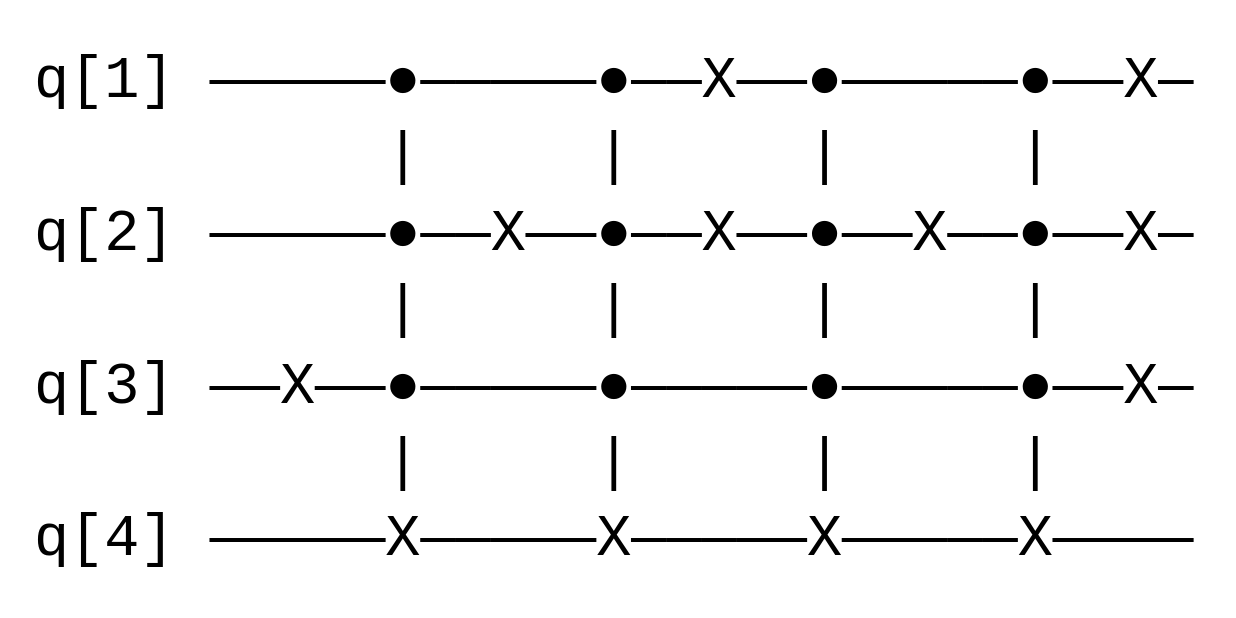
\includegraphics[width=0.4\textwidth]{algebraic circuits/dj1_qc.png}}
            \caption{Graphical Representation of Unoptimised Deutsch-Jozsa Circuit.}
            \label{dj1_qc}
        \end{figure}

        \item Graphical representation of the optimised circuit (Fig.~\ref{dj2_qc}).
        \begin{figure}[!ht]
            \centerline{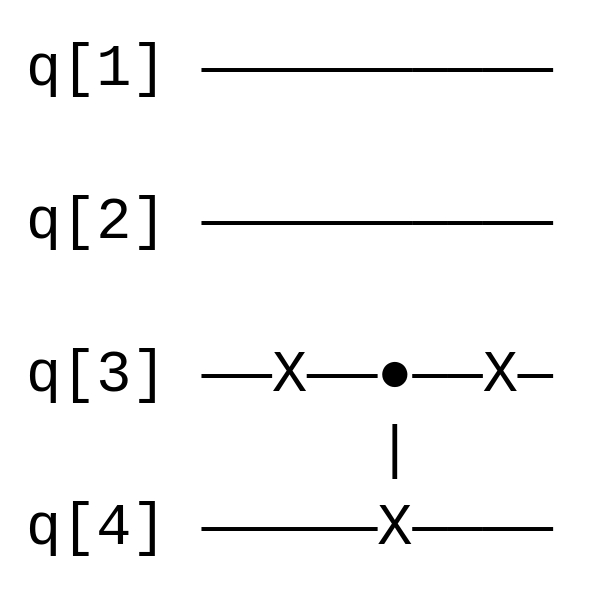
\includegraphics[width=0.18\textwidth]{algebraic circuits/dj2_qc.png}}
            \caption{Graphical representation of Optimised Deutsch-Jozsa Circuit.}
            \label{dj2_qc}
        \end{figure}
\end{enumerate}

\section{Conclusions and Future Works}
In this paper a notation with great potential to represent quantum circuits from an algebraic point of view has been proposed. This new notation greatly facilitates the discovery and proof of new properties and relationships between quantum gates, as well as the handling of calculations and the efficiency of systems that simulate them classically. To show it, a computer tool has been developed that is able to simulate in a classical way the evolution of the state vector through a circuit expressed in algebraic notation. Several examples are shown that clarify the results and consolidate the idea of easier handling of circuits in algebraic notation, compared to the traditional graphical representation. %Several definitions and propositions have been established using this new language, providing an initial framework from which to start investigating this new paradigm. 

Three future lines of  research are the following: to extend the notation to add higher level abstraction features, to find properties that simplify the patterns most used in the development of quantum algorithms, and to introduce the concept of measurement (both in notation and implementation).    
This last issue is relevant because the focus now is on the evolution of the state vector, without actually measuring it.  These lines can enhance the growth of the theoretical basis and the proposed implementation, leading to the creation of a new manageable language for the characterization of quantum circuits. Finally, it is also proposed to migrate the existing implementation to the Rust language, where a more efficient way to compute the final state vector is already being designed and developed.
